


\section{Blowing up the tails and
constructing\\ $\mathcal{H}_{2}^\diamond, \mathcal{H}_{3}^\diamond, 
\ldots, \mathcal{H}_{n}^\diamond=\mathcal{H}_{n}^\star$}

The process of replacing the embedded tail of a balloon by the corresponding
trio of PL2-faces in the pillow is denominated \index{blow up a tail} {\em the blowing up of the 
balloon's tail}.

%{\huge \bf Aqui insira seus $\alpha, \beta, \gamma$, bumps, etc}
%\begin{theorem}\label{theo:teoremadeumalinha}
% There is an $O(n)$-algorithm for blowing up a single balloon's tail.
%Thus finding $E\mathcal{L}_n^\star$ and  $E\mathcal{H}_n^\star= 
%E\mathcal{U}_n^\star \cup E\mathcal{L}_n^\star$
%take $O(n^2)$ steps.
%\end{theorem}
\begin{theorem}\label{theo:teoremadeumalinha}
 There is an $O(n)$-algorithm for blowing up a single balloon's tail.
Thus finding $\mathcal{H}_n^\star$ take, $O(n^2)$ steps.
\end{theorem}
\begin{proof}
%Here we get an explicit embedding $E\mathcal{L}_{n}^\star$.
%This finishes the description of $E\mathcal{H}_n^\star.$
%This 2-complex becomes geometrically
%consistent with the combinatorial one in the sense 
%that there are no spurious crossings. 
$\mathcal{H}_{i+1}^\diamond$ is the union of $\mathcal{H}_{i}^\diamond$ with $\mathcal{L}_{i+1}^\star$
and an {\em $\epsilon$-change} in some PL3-faces, if the rank of the type of balloon's tail of the i-th $bp$-move has rank greater than 1
(we call $\epsilon$-change because this change is small, as described below).
At the same time we update the colors of the middle layer to match the colors of the $i$-th pillow in the sequence of $bp$-moves.


%(We proceed the embed of $\mathcal{L}_i^\star$ in the same order as the $bp$-move.
%In each step from $E\mathcal{U}_i^\star$ to $E\mathcal{U}_{i+1}^\star$,
% we change the color of two 2-simplices in the medial layer, of the open balloon's head of this step in $E\mathcal{U}_i^\star$,
%to match with the medial layer of the $bp$-move and embed $\mathcal{L}_i^\star$.
%Basically $E\mathcal{U}_{i+1}^\star$ is the union of $E\mathcal{U}_{i}^\star$ with 
%$E\mathcal{L}_{i}^\star$ and a change of the color in two 2-simplices of $\mathcal{U}_{i}^\star$
%(in some steps we make changes in some tetrahedra which is already embedded to create space to the embed of $\mathcal{L}_i^\star$).
% The final embedding $E\mathcal{U}_n^\star$ is equals to $E\mathcal{H}_n^\star$,
%but $E\mathcal{U}_i^\star \neq E\mathcal{H}_i^\star$ if $i<n.$

Now we describe how to embed each kind of $\mathcal{L}_{i}^\star$ 
(explaining how to $\epsilon$-change some PL3-faces,
to get space for $E\mathcal{L}_i^\star$).


If the balloon's tail is of type $P_1$ (the case $B_1$ is analogous).
Make two copies of $P_1$, resulting in three $P_1$, but change the color of the one which will be in
the middle, and define the 0-simplices like in Fig. \ref{fig:3d2}.

\begin{figure}[!htb] 
\begin{center}
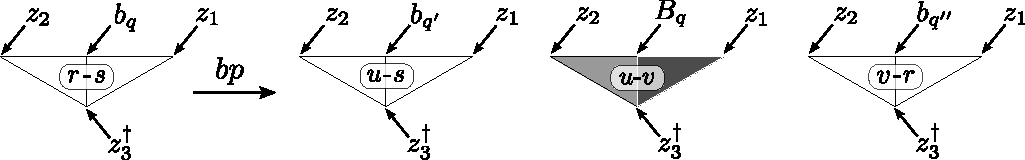
\includegraphics[width=14cm]{A.figs/3d2.pdf}
\caption{Embedding the part of the pillow corresponding to the tail of the balloon: case $P_1$ of the tail.}
\label{fig:3d2}
\end{center}
\end{figure}
If the balloon's tail is of type $B_i$, $i>1$ (the case $P_i$ is analogous).
Make two copies of $B_i$, refine the copies and the original, resulting in three $B_i'$, 
but change the color of the one which will be in
the middle, and define the 0-simplices like in Fig. \ref{fig:3d3}.


The images $\chi_j$ we already know from previous $bp$-move, now we need to define all the images
$\alpha_j, \beta_j$ and $\gamma_j.$
Let $\beta_j$ be $\frac{z_2+\chi_{j+1}}{2}$ 
for each $j=1,\ldots, i$.
As the images $\alpha_j$ and $\gamma_j$ can be defined in analogus way, we just explain how to define each $\alpha_j$.
We know that each $\alpha_j$ is in the PL3-face $\nabla_r$. To 
define each $\alpha_j$ we need 
to reduce the PL3-face $\nabla_r$
in order to get enough space for the PL2-faces of color 0 and 2 of the PL3-faces $\nabla_u$ and $\nabla_v$.
Consider the PL3-face $\nabla_r$, each $\beta_j$ is already defined, so 
define each $\zeta_j$ as $\frac{z_2+\omega_{j+1}}{2}$, where $\omega_k$ is previously defined, %that they are as if we where going to refine
 see Fig. \ref{fig:nextdual3}. Define $\alpha_j$ as $\frac{\zeta_j+\beta_j}{2}$. 

\begin{figure}[!htb] 
\begin{center}
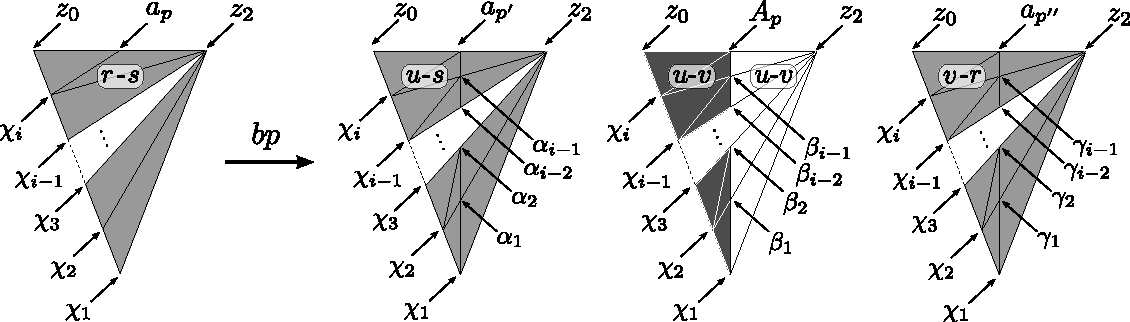
\includegraphics[width=14cm]{A.figs/3d3.pdf}
\caption{Embedding the part of the pillow corresponding to the tail of the balloon: case $B_i$ of the tail.}
\label{fig:3d3}
\end{center}
\end{figure}

\begin{figure}[!htb] 
\begin{center}
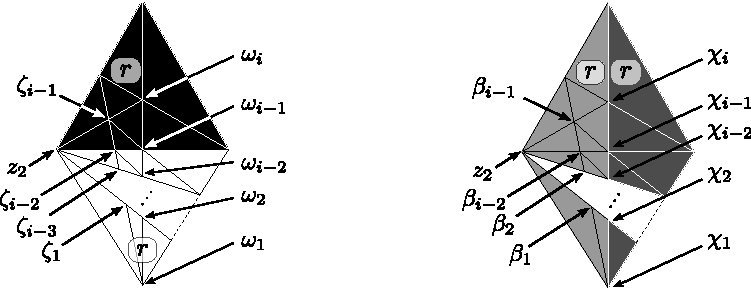
\includegraphics[scale=0.8]{A.figs/nextdual3.pdf}
\caption{Using the PL3-face corresponding to $r$ to define the $\alpha_j$ as $\frac{\zeta_j+\beta_j}{2}$.}
\label{fig:nextdual3}
\end{center}
\end{figure}


The last case is when balloon's tail is refined, that means it is of type $P_i'$ or $B_i'$, $i>1$. We treat the case $B_i'$,
 see Fig. \ref{fig:3d4}. All the 0-simplices $\beta_j$ are already defined, we need to define each
$\alpha_j$ and each $\gamma_j$. Observe that here $r\neq s-1$ and the definitions of $\alpha_j$ and $\gamma_j$ 
are not analogous.

\begin{figure}[!htb] 
\begin{center}
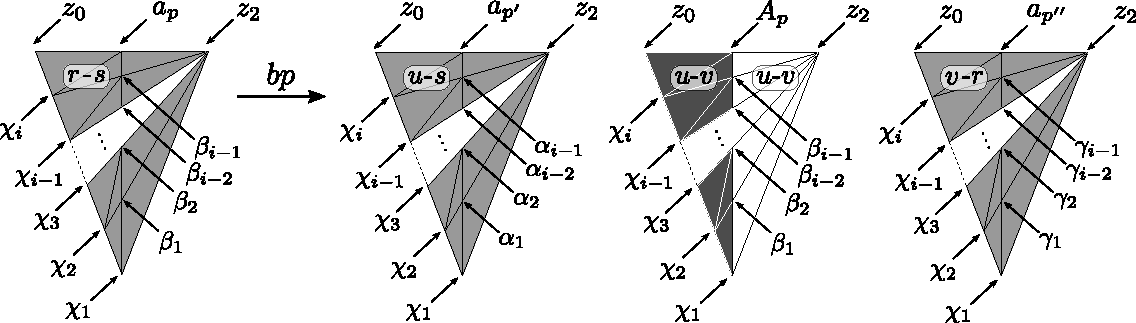
\includegraphics[width=15cm]{A.figs/3d4.pdf}
\caption{Embedding the part of the pillow corresponding to the tail of the balloon: case $B_i'$ of the tail.}
\label{fig:3d4}
\end{center}
\end{figure}


In this case, we need to reduce the PL3-faces $\nabla_r$ and $\nabla_s$
to create enough space to build PL2-faces 0- and 2-colored.
To define 0-simplices $\alpha_j$ and $\gamma_j$, one of these cases is analogous to the case not
 refined, but the other we describe here. ($\nabla_r$ is in the new case is the rank 
%of
%the PL2$_0$- and PL2$_1$-faces of $\nabla_r$, the new case 
%happens when the rank
 of PL2$_0$-face is equals to the rank of the PL2$_1$-face plus 2, if its not true,
the new case is in the PL3-face $\nabla_v$).
Suppose that the new case is in the PL3-face, $\nabla_r$. To define $\alpha_j$,
suppose that the PL2$_0$-face of this PL3-face is not refined,
 see Fig. \ref{fig:3d5}. Define each $\alpha_j$  as the middle point between $\beta_j$ and $\omega_j$.



\begin{figure}[!htb] 
\begin{center}
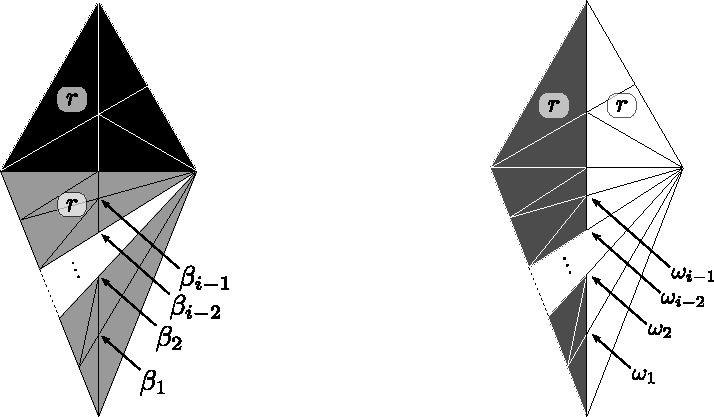
\includegraphics[scale=0.7]{A.figs/3d5.pdf}
\caption{Using the PL3-face $\nabla_r$ to define $\alpha_j$ as $\frac{\omega_j+\beta_j}{2}$.}
\label{fig:3d5}
\end{center}
\end{figure}

Consider the case that the PL2$_0$-face, of the PL3-face $\nabla_r$, is refined
see Fig. \ref{fig:3d6}.
 This is a final subtlety which 
is treated with the {\em bump}. \index{bump} This is characterized by a
non-convex pentagon shown in the bottom part of Fig. \ref{fig:3d6}.
Let $\nu_j$ be $\frac{z_2+\omega_j}{2}$
and $\alpha_j$ as $\frac{\beta_{j-1}+\nu_j}{2}$, for $j=1,\ldots, i-1$. Observe that
if we define $\alpha_j$ as if the PL2$_0$-face
where not refined, some 1-simplices may cross.

%\begin{figure}[!htb] 
%\begin{center}
%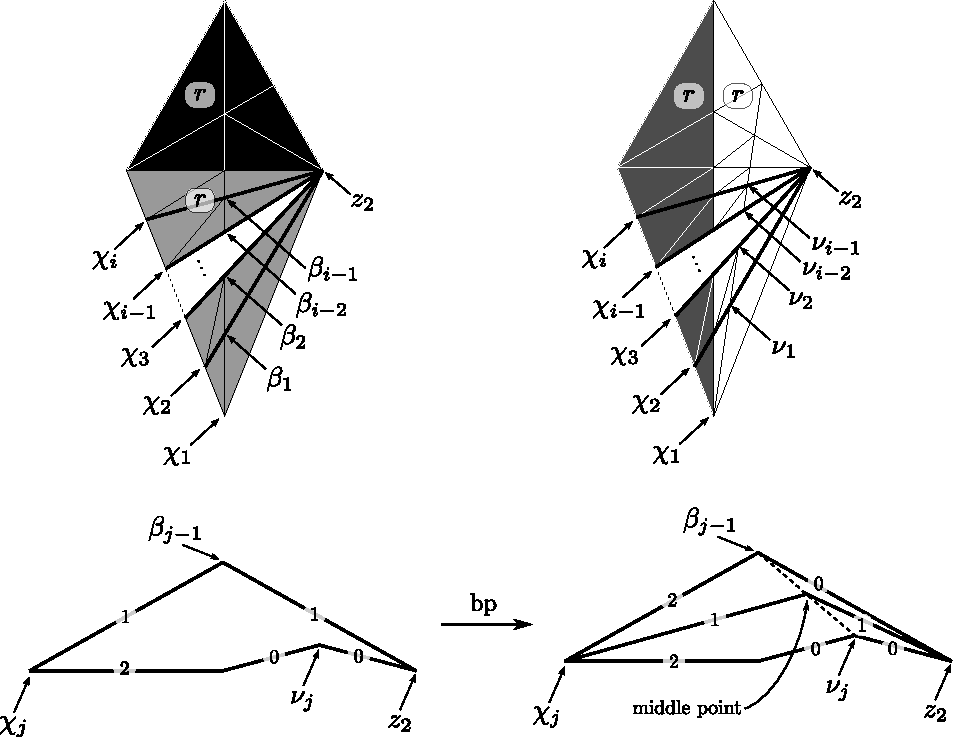
\includegraphics[scale=0.7]{A.figs/3d6.pdf}
%\caption{Using the PL-tetrahedron $\nabla_r$ to define $\alpha_j$ as the middle point between $\mathcal{\nu}_j$ and $\beta_{j-1}$
%(because of the bump, see Fig. \ref{fig:3d7}).}
%The bump: a final dificulty to overcome.}
%\label{fig:3d6}
%\end{center}
%\end{figure}


\begin{figure}[!htb] 
\begin{center}
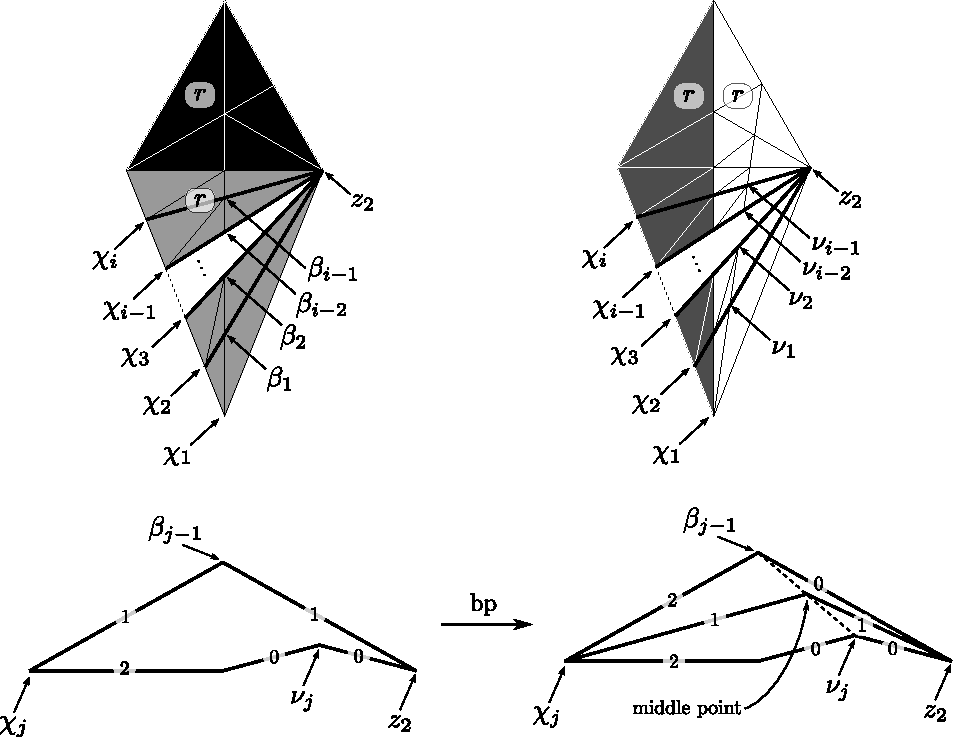
\includegraphics[scale=0.7]{A.figs/3d6.pdf}
\caption{The bump: a final subtlety and how to deal with it.}
\label{fig:3d6}
\end{center}
\end{figure}

\end{proof}
